\chapter[Sequential models: RNN, LSTM, GRU, Transformers]{Sequential and Attention models: RNN, LSTM, GRU, Transformers}
%--------------------------------------------------------

%-----------------------Sequence models (I gruppo di slides)------------
\begin{quotation}
    \noindent
    \textsf{In this chapter we will discuss about some tasks that according to their features requires special neural network architectures that are something different with respect to the model we have already seen talking about MLP and ConvNet for computer vision activities. We are talking about \textit{Recurrent Neural Network (RNN)}, such models are used in order to perform computation on  \textit{time series data}. \textbf{Time} is the new component to handle. The related tasks include: speech recognition, music generation, DNA sequence analysis and so on. After some prerequisites, we are introducing RNN and more robust architectures (\textit{LSTM, GRU}). Finally the state-of-art architecture for NLP is analyzed (\textit{Transformer}).  
    }
\end{quotation}

\begin{figure}[h]
    \centering
    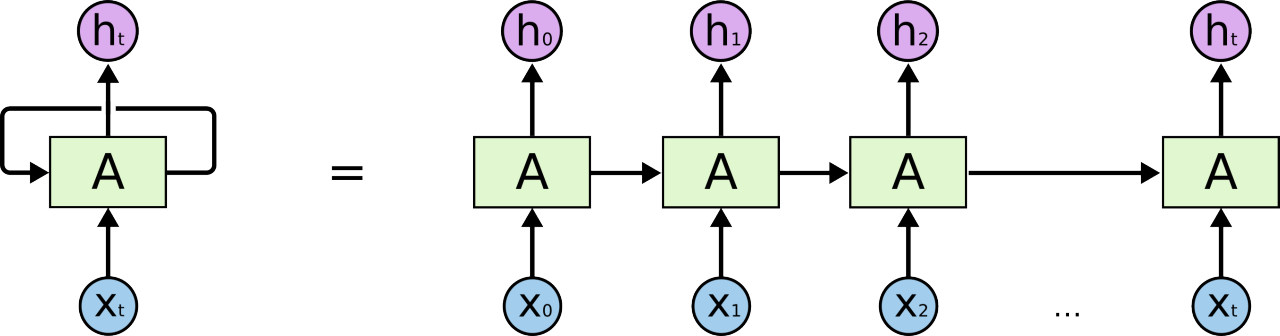
\includegraphics[scale=0.3]{img/rnn_1.png}
\end{figure}

\section{Notation}
In order to introduce some \textbf{notation}, we use a practical example. In the field of information extraction in the context of \textit{Natural Language processing (NLP)}, there is a sub-task which is called \textbf{Named entity recognition}, this deals with the classification of the name appearing in a sentence according to predetermined categories.
Suppose you want to recognize the person name in the sentence:
\begin{center}
    \textit{Harry Potter and Hermione Granger invented a new spell}
\end{center}
This is a sequence of words constituting a phrase. We need a notation in order to handle the concept of \textit{sequentiality}. One possibility is to use for the words, which will be the input of our models (anyhow they are made), the notation
\begin{equation*}
    x=\{x^{<1>}\quad x^{<2>} \quad ... \quad x^{<T_x>}\}
\end{equation*}  
Indicating with an index the \textit{time at which the word appear in the sentence}. The size of the input sample $x$ is $T_x$. The same reasoning holds for the output $y$, which is suggesting us, the words related to name of person. In the specific case we will have
\begin{equation*}
    y=\{y^{<1>}, y^{<2>}, \dots, y^{<T_y>}\} = \{1,1,0,1,1,0,0,0,0\}
\end{equation*}
Since \textit{Harry Potter} and \textit{Hermion Granger} are the names in the given sequence. It is not said that $T_x$ and $T_y$ are of the same length. The concept of \textbf{time} is a novelty with respect to the other tasks we have seen. Sequentiality makes necessary the introduction of new aspects we have not considered till now. Let us start!

\section{Representing words}
It is not a novelty if we say that Neural networks manage effectively numbers by doing several forms of computation in order to perform their task. Well, even in the presence of sequential data, we have to map them in some "numeric space", first of all the \textbf{words}. \\

When we are dealing with NLP, mostly, there is a \textbf{dictionary} with a great number of words which can be used in the analysis. Then, if we have examples made up of phrases, each word is mapped into a \textit{sparse vector} in which \textbf{only the number at the position where the word itself is located in the vocabulary is one}, all the other numbers are 0. For this reason such an encoding is called \textbf{one-hot encoding}. 
Such a work is carried out after that the sentences have been \textbf{tokenized}\footnote{
    Sometimes, for certain types of computation, the \textbf{stemming} is preferred; this is the process by which each word is recasted to its \textit{root form}.
}. \\
To tell the truth the architectures we are going to see, do not take into account this sparse representation, at least directly. Differently, often the words during the training of \textit{language models} are mapped into an \textit{hyperdimensional dense space} in the so-called \textbf{word embeddings} which are succint synthesis of the general meaning for a certain word. Such encoding can be pretrained or fine tuned or made by scratch in some cases, being included into the \textit{trainable parameters}. Anyway, \textit{one-hot encodings} are important since they are fed into an \textit{embedding lookup module} which will provide the inputs $x$ to the NN. To conclude this part, let us provide an example. We want the one-hot encodings for the word \textit{cat}, while the voabulary is: 
\begin{align*}
    \text{Vocabulary} =\{ a,\ aaron, \ ..., \  aerospace, \ cat, \ ..., \  zulu\}
\end{align*}
The one-hot encoding is:
\begin{equation*}
    [0, \ 0, \ ... \ 0, \ 1, \ ..., 0]
\end{equation*}

\section{Recurrent Neural Networks (RNN)}
\subsection{Motivations for introducing a novel architecture}
Everytime we have to introduce a new architecture, it is quite natural asking ourself: \textit{Can we use, instead, the architectures we already have?} There are several reasons for which the answer is NO.
\begin{enumerate}
    \itemsep-0.2em
    \item In models dealing with sequential data, the \textbf{size} of input/output \textbf{can be different} in different samples.
    \item Standard NNs do not share the features learned across the different position of the sequence; 
    \item Standard NNs, first of all, do not include \textit{ memory mechanisms} which are fundamental here, due to the presence of \textit{sequentiality}
\end{enumerate}

\subsection{Recurrent neurons and layers}
Up to now we have seen models where the outputs flowed only in one direction: forward. A \textbf{recurrent neural network} has more or less the same structure of a Feed-forward Neural Network, except the fact it have \textbf{backward connections}. \\
The simplest possible RNN is the one made up of \textit{one neuron} that receive the input, produce the output and send its output, or in more complex situations, its \textbf{hidden state}, back to itself. When the first input is received this output/hidden state is usually initialized to 0 since the network has not already produced any output. As showed in \Cref{fig:r_neuron} the recurrent neuron can be represented \textit{against the time axis} in the so-called \textbf{unrolled representation} (it's the same recurrent neuron once per time step).

\begin{figure}[h]
    \centering
    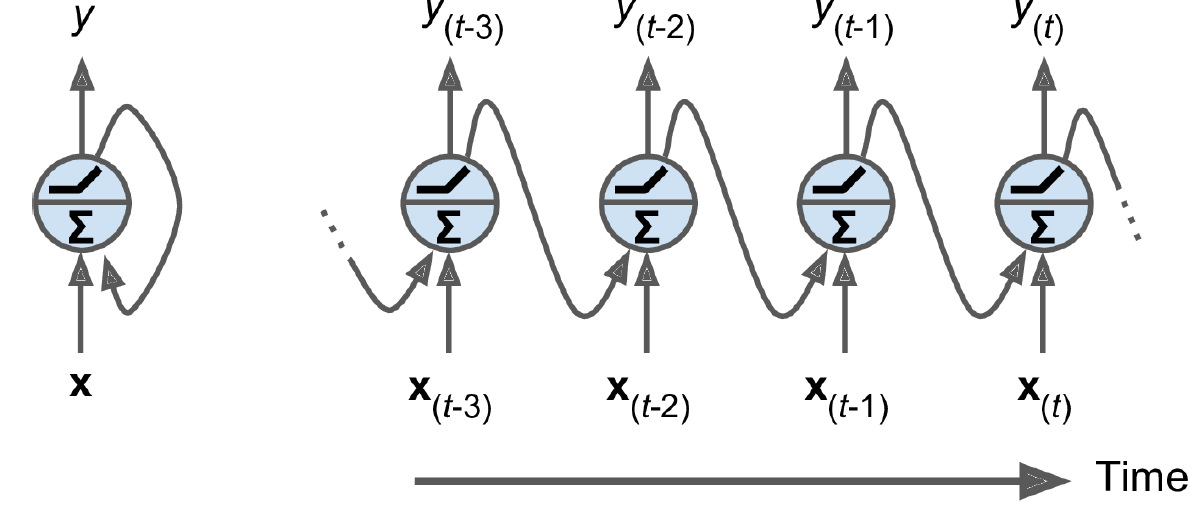
\includegraphics[scale=0.5]{img/rnn.png}
    \caption{Recurrent neuron}
    \label{fig:r_neuron}
\end{figure}
\noindent
Here, it is even more clear that for each time instant the neuron, receives not only the input $x$ but also another information coming from past computations. The output of such a \textit{tiny network} is simply a scalar.\\
It is quite simple to extend the reasoning we have done for a \textbf{layer recurrent neurons} where each neuron receives the input and the \textbf{backward information}. Here the output is a vector, since there many neurons. A \textit{recurrent layer} together with its unrolled representation is showed in the \Cref{fig:r_layer}.

\begin{figure}
    \centering
    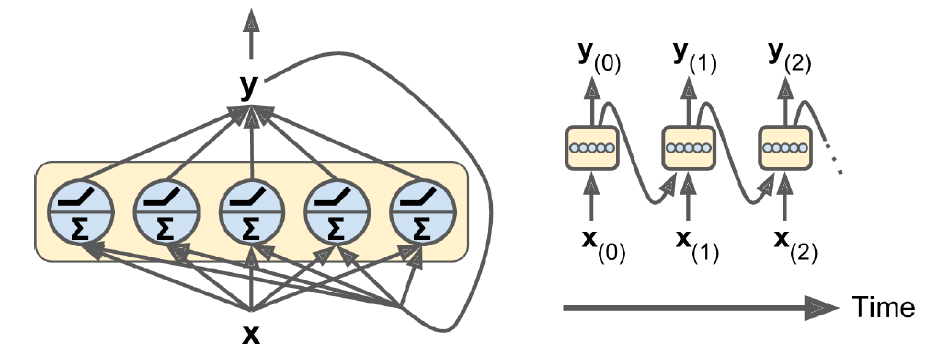
\includegraphics[scale=0.7]{img/rnn_layer.png}
    \caption{Recurrent layer}
    \label{fig:r_layer}
\end{figure}

Since the output of a recurrent neuron at time step $t$ is a function of all the inputs from previous time steps, this is the reason why we refer to recurrent architecture by using the term \textbf{memory cell}. In the examples we have analyzed of recurrent neuron and layer, we have assumed that the backward information was the output, in more complex architectures this is not the case, but we call it \textbf{hidden state}, we are indicating it with the notation $h^{<t>}$.\\
Each neuron has \textbf{three sets of weights}: 
\begin{enumerate}
    \itemsep-0.2em
    \item $w_{hx}$ from the input to the hidden state; 
    \item $w_{hh}$ from one hidden state and the following; 
    \item $w_{ya}$ from the hidden state to the output
\end{enumerate} 
Since we have multiple neurons we can group such weights in matrices, like we did for feedforward architectures. Then, we have $W_{hx}$, $W_{hh}$ and $W_{ya}$. 

\subsubsection{Forward propagation}

\subsubsection{Backward propagation}

\subsection{RNN architectures}

\subsection{Bidirectional RNN}

\subsection{Deep RNN}

\section{Language Modeling with RNN}

\section{Issues with RNN training}

\section{Long-Short Term memories (LSTM)}

\section{Gated Recurrent Unit (GRU)}


%--------------Attention models (II gruppo di slides)------------------
%\section{Application: Image captioning}

%\section{Attention mechanisms}

%\section{Transformers: Attention is all you need}